\documentclass[12pt, titlepage]{article}

\usepackage{fullpage}
\usepackage[round]{natbib}
\usepackage{multirow}
\usepackage{booktabs}
\usepackage{tabularx}
\usepackage{graphicx}
\usepackage{float}
\usepackage{hyperref}
\hypersetup{
    colorlinks,
    citecolor=black,
    filecolor=black,
    linkcolor=red,
    urlcolor=blue
}
\usepackage[round]{natbib}

\newcounter{acnum}
\newcommand{\actheacnum}{AC\theacnum}
\newcommand{\acref}[1]{AC\ref{#1}}

\newcounter{ucnum}
\newcommand{\uctheucnum}{UC\theucnum}
\newcommand{\uref}[1]{UC\ref{#1}}

\newcounter{mnum}
\newcommand{\mthemnum}{M\themnum}
\newcommand{\mref}[1]{M\ref{#1}}

\title{SE 3XA3: Software Requirements Specification\\GoDBMS}

\author{Team \#7, Databased
		\\ Eesha Qureshi, qureshe 
		\\ Faiq Ahmed, ahmedf46 
		\\ Kevin Kannammalil, kannammk
}

\date{\today}

\begin{document}

\maketitle

\pagenumbering{roman}
\tableofcontents
\listoftables
\listoffigures

\begin{table}[H]
\caption{\bf Revision History}
\begin{tabularx}{\textwidth}{p{3cm}p{2cm}X}
\toprule {\bf Date} & {\bf Version} & {\bf Notes}\\
\midrule
March 17 & 1.0 & Started assignment\\
March 17 & 1.1 & Created Modules\\
March 18 & 1.2 & Created Modules Heirarchy Diagram\\
March 18 & 1.3 & Finished Document\\
\bottomrule
\end{tabularx}
\end{table}

\newpage

\pagenumbering{arabic}

\section{Introduction}

GoDBMS is a database management software based on the project SimpleDB. The aim of GoDBMS is to develop a software that maintains the basic functionality of SimpleDB but has a lighter weight, optimizes memory usage, has a simpler code base and is developed using GoLang. This project will be properly documented and iteratively developed following the Software Development Life Cycle.

\subsection{Purpose}

The purpose of this document is to provide insight into the modular decomposition of the system. This will allow for developers and other intended audience to understand each component in the system and how it connects in the system architecture, the module hierarchy, and information hiding between modules. 

\subsection{Scope}
This document provides detail about the modular decomposition and relational hierarchy of the modules that comprise the system. In contrast, the MIS will provide specifications about the behaviour of each module and component.


\subsection{Acronyms, Abbreviations, and Symbols}
\begin{table}[H]
\caption{\bf Revision History}
\begin{tabularx}{\textwidth}{p{3cm}p{2cm}X}
\toprule {\bf Term} & {\bf Abbreviation} & {\bf Definition}\\
\midrule
Database Management System & DBMS & Software used to manage database transactions and operations\\
Structured Query Language & \textbf{SQL} & Language used to write database transaction instructions\\
Command Line Interface & \textbf{CLI} & Point of contact between user and computer instructions \\
\textbf{Catalog} & N/A & A list storing the names of all the tables in the database. This list can be encoded and decoded from a file to allow persistent storage.\\
\textbf{Record} & N/A & A single row of data in a database\\
Heap File & N/A & A basic data structure that uses memory blocks and stores new files at the end \\
Encoder & N/A & Resolves the mapping between items \\
Lock & N/A  & Data variables that synchronize concurrent transactions \\
\textbf{HTTP Server} & N/A & Information transfer protocol for the internet \\

\bottomrule
\end{tabularx}
\end{table}

\subsection{Overview of Document}
This document will highlight anticipated changes to the system, as well as unlikely changes. Then it will delve into the module hierarchy, followed by comparisons between the requirements and design. Next it will present the modular decomposition of the system in great detail. Finally, this document will provide a traceability matrix and summarize the use hierarchy between modules.
\section{Anticipated and Unlikely Changes} \label{SecChange}

This section lists possible changes to the system. According to the likeliness
of the change, the possible changes are classified into two
categories. Anticipated changes are listed in Section \ref{SecAchange}, and
unlikely changes are listed in Section \ref{SecUchange}.

\subsection{Anticipated Changes} \label{SecAchange}

Anticipated changes are the source of the information that is to be hidden
inside the modules. Ideally, changing one of the anticipated changes will only
require changing the one module that hides the associated decision. The approach
adapted here is called design for
change.

\begin{description}
\item[\refstepcounter{acnum} \actheacnum \label{ac1}:] The directory where the \textbf{DBMS} is installed
\item[\refstepcounter{acnum} \actheacnum \label{ac2}:] The method to store the \textbf{record}s
\item[\refstepcounter{acnum} \actheacnum \label{ac3}:] The method of interfacing with the \textbf{DBMS}
\item[\refstepcounter{acnum} \actheacnum \label{ac4}:] The styling of the command line interface and displayed messages
\item[\refstepcounter{acnum} \actheacnum \label{ac5}:] The supported \textbf{SQL} commands in the \textbf{DBMS}
\item[\refstepcounter{acnum} \actheacnum \label{ac6}:] The supported \textbf{SQL} data types in the \textbf{DBMS}
\item[\refstepcounter{acnum} \actheacnum \label{ac7}:] The structure of the \textbf{catalog}.
\end{description}

\subsection{Unlikely Changes} \label{SecUchange}

The module design should be as general as possible. However, a general system is
more complex. Sometimes this complexity is not necessary. Fixing some design
decisions at the system architecture stage can simplify the software design. If
these decision should later need to be changed, then many parts of the design
will potentially need to be modified. Hence, it is not intended that these
decisions will be changed.

\begin{description}
\item[\refstepcounter{ucnum} \uctheucnum \label{uc1}:] Input/Output devices since interacting with a database only requires the use of a keyboard.
\item[\refstepcounter{ucnum} \uctheucnum \label{uc2}:] The encoding and decoding of \textbf{DBMS} persistent data.
\item[\refstepcounter{ucnum} \uctheucnum \label{uc3}:] The \textbf{DBMS} will always take in strings as input queries.
\end{description}

\section{Module Hierarchy} \label{SecMH}

This section provides an overview of the module design. Modules are summarized
in a hierarchy decomposed by secrets in Table \ref{TblMH}. The modules listed
below, which are leaves in the hierarchy tree, are the modules that will
actually be implemented.

\begin{description}
\item [\refstepcounter{mnum} \mthemnum \label{m1}:] \textbf{CLI}
\item [\refstepcounter{mnum} \mthemnum \label{m2}:] Controller
\item [\refstepcounter{mnum} \mthemnum \label{m3}:] Parser
\item [\refstepcounter{mnum} \mthemnum \label{m4}:] Parse Modify \textbf{Record}
\item [\refstepcounter{mnum} \mthemnum \label{m5}:] Parse Insert \textbf{Record}
\item [\refstepcounter{mnum} \mthemnum \label{m6}:] Parse Create Table
\item [\refstepcounter{mnum} \mthemnum \label{m7}:] Parse Delete Table
\item [\refstepcounter{mnum} \mthemnum \label{m8}:] Parse Delete \textbf{Record}
\item [\refstepcounter{mnum} \mthemnum \label{m9}:] Parse Select
\item [\refstepcounter{mnum} \mthemnum \label{m10}:] Process \textbf{SQL} Statements
\item [\refstepcounter{mnum} \mthemnum \label{m11}:] Storage Lock
\item [\refstepcounter{mnum} \mthemnum \label{m12}:] Storage Encoder
\item [\refstepcounter{mnum} \mthemnum \label{m13}:] Heap File
\item [\refstepcounter{mnum} \mthemnum \label{m14}:] \textbf{Catalog}
\item [\refstepcounter{mnum} \mthemnum \label{m15}:] \textbf{Catalog} Encoder
\item [\refstepcounter{mnum} \mthemnum \label{m16}:] File Management
\end{description}


\begin{table}[h!]
\centering
\begin{tabular}{p{0.3\textwidth} p{0.6\textwidth}}
\toprule
\textbf{Level 1} & \textbf{Level 2}\\
\midrule

{Hardware-Hiding Module} & ~ \\
\midrule

\multirow{7}{0.3\textwidth}{Behaviour-Hiding Module} & \textbf{CLI}\\
& Parser\\
& Storage Encoder\\
& \textbf{Catalog} Encoder\\
& File Management\\
\midrule

\multirow{3}{0.3\textwidth}{Software Decision Module} & Controller\\
& Parse Modify \textbf{Record}\\
& Parse Insert \textbf{Record}\\
& Parse Create Table\\
& Parse Delete Table\\
& Parse Delete \textbf{Record}\\
& Parse Select\\
& Process \textbf{SQL} Statements\\
& Storage Lock\\ 
& Heap File\\
& \textbf{Catalog}\\
\bottomrule

\end{tabular}
\caption{Module Hierarchy}
\label{TblMH}
\end{table}

\section{Connection Between Requirements and Design} \label{SecConnection}

The design of the system is intended to satisfy the requirements developed in
the SRS. In this stage, the system is decomposed into modules. The connection
between requirements and modules is listed in Table \ref{TblRT}.

\section{Module Decomposition} \label{SecMD}

Modules are decomposed according to the principle of ``information hiding''
proposed by Parnas. The \emph{Secrets} field in a module
decomposition is a brief statement of the design decision hidden by the
module. The \emph{Services} field specifies \emph{what} the module will do
without documenting \emph{how} to do it. For each module, a suggestion for the
implementing software is given under the \emph{Implemented By} title. If the
entry is \emph{OS}, this means that the module is provided by the operating
system or by standard programming language libraries.  Also indicate if the
module will be implemented specifically for the software.

Only the leaf modules in the
hierarchy have to be implemented. If a dash (\emph{--}) is shown, this means
that the module is not a leaf and will not have to be implemented. Whether or
not this module is implemented depends on the programming language
selected.

\subsection{Hardware Hiding Modules}
N/A

\subsection{Behaviour-Hiding Module}

\subsubsection{\textbf{CLI} (\mref{m1})}
\begin{description}
\item[Secrets:]Method to get user input and print back output to the user.
\item[Services:]Gets the user input from a the command line and sends it to the \textbf{DBMS} using a http request. Prints back the output of the request back to the user.
\item[Implemented By:] Go\textbf{DBMS}
\end{description}

\subsubsection{Parser (\mref{m3})}
\begin{description}
\item[Secrets:]Method to retrieve appropriate query fields for each statement from a string input.
\item[Services:]Takes a string input and parses the necessary information from the string that is specific to the \textbf{SQL} statement.
\item[Implemented By:] Go\textbf{DBMS}
\end{description}

\subsubsection{Storage Encoder (\mref{m12})}
\begin{description}
\item[Secrets:]Method to convert a \textbf{heap file} into a byte array and convert a byte array into a \textbf{heap file}.
\item[Services:]Loads or saves a Heap File.
\item[Implemented By:] Go\textbf{DBMS}
\end{description}

\subsubsection{\textbf{Catalog} Encoder (\mref{m15})}
\begin{description}
\item[Secrets:]Method to convert a \textbf{catalog} array into a byte array and convert a byte array into a \textbf{catalog} array.
\item[Services:]Loads or saves the \textbf{Catalog}.
\item[Implemented By:] Go\textbf{DBMS}
\end{description}

\subsubsection{File Management (\mref{m16})}
\begin{description}
\item[Secrets:]Path of directory for save files, methods to load and save files.
\item[Services:]Is able to save a byte array into a data file in the save files directory and load a byte array from a data file in the save files directory.
\item[Implemented By:] Go\textbf{DBMS}
\end{description}

\subsection{Software Decision Module}

\subsubsection{Controller (\mref{m2})}
\begin{description}
\item[Secrets:]Method to get the type of \textbf{SQL} command from string input and the connection between the parser and processing \textbf{SQL} statements.
\item[Services:]Gets a string value from the \textbf{HTTP Server} and gets the correct command type before sending it to the appropriate parser function. Takes the return value of the parser function and sends the relevant information to be processed. This module also returns all outputs and errors back to the \textbf{HTTP Server}.
\item[Implemented By:] Go\textbf{DBMS}
\end{description}

\subsubsection{Parse Modify \textbf{Record} (\mref{m4})}
\begin{description}
\item[Secrets:]Modify \textbf{Record} Statement Information
\item[Services:]This module has a constructor for the modify \textbf{record} structure which contains all the relevant information about the modify \textbf{record} statement.
\item[Implemented By:] Go\textbf{DBMS}
\end{description}

\subsubsection{Parse Insert \textbf{Record} (\mref{m5})}
\begin{description}
\item[Secrets:]Modify Insert Statement Information
\item[Services:]This module has a constructor for the insert \textbf{record} structure which contains all the relevant information about the insert \textbf{record} statement.
\item[Implemented By:] Go\textbf{DBMS}
\end{description}

\subsubsection{Parse Create Table (\mref{m6})}
\begin{description}
\item[Secrets:]Create Table Statement Information
\item[Services:]This module has a constructor for the create table structure which contains all the relevant information about the create table statement.
\item[Implemented By:] Go\textbf{DBMS}
\end{description}

\subsubsection{Parse Delete Table (\mref{m7})}
\begin{description}
\item[Secrets:]Delete Table Statement Information
\item[Services:]This module has a constructor for the delete table structure which contains all the relevant information about the delete table statement.
\item[Implemented By:] Go\textbf{DBMS}
\end{description}

\subsubsection{Parse Delete \textbf{Record} (\mref{m8})}
\begin{description}
\item[Secrets:]Delete \textbf{Record} Statement Information
\item[Services:]This module has a constructor for the delete \textbf{record} structure which contains all the relevant information about the delete \textbf{record} statement.
\item[Implemented By:] Go\textbf{DBMS}
\end{description}

\subsubsection{Parse Select (\mref{m9})}
\begin{description}
\item[Secrets:]Select Statement Information
\item[Services:]This module has a constructor for the select structure which contains all the relevant information about the select statement.
\item[Implemented By:] Go\textbf{DBMS}
\end{description}

\subsubsection{Process \textbf{SQL} Statements (\mref{m10})}
\begin{description}
\item[Secrets:]The logic to modify the storage of the database appropriately according to each \textbf{SQL} statement.
\item[Services:]Modifies the storage of the database and the \textbf{catalog} according to which function in this module is called and what parameters are passed in.
\item[Implemented By:] Go\textbf{DBMS}
\end{description}

\subsubsection{Storage Lock (\mref{m11})}
\begin{description}
\item[Secrets:]The semaphore \textbf{lock}s for each table.
\item[Services:]Allows a \textbf{lock} for a table to be acquired or released.
\item[Implemented By:] Go\textbf{DBMS}
\end{description}

\subsubsection{Heap File (\mref{m13})}
\begin{description}
\item[Secrets:]String \textbf{record}s that are in the current table
\item[Services:]Saves new \textbf{record}s, removes \textbf{record}s, modifies \textbf{record}s, or allows searching for \textbf{record}s.
\item[Implemented By:] Go\textbf{DBMS}
\end{description}

\subsubsection{\textbf{Catalog} (\mref{m14})}
\begin{description}
\item[Secrets:]List of all tables in the database and how they are stored.
\item[Services:]Saves new tables, deletes tables, and allows searching for table information.
\item[Implemented By:] Go\textbf{DBMS}
\end{description}

\section{Traceability Matrix} \label{SecTM}

This section shows two traceability matrices: between the modules and the
requirements and between the modules and the anticipated changes.

% the table should use mref, the requirements should be named, use something
% like fref
\begin{table}[H]
\centering
\begin{tabular}{p{0.6\textwidth} p{0.2\textwidth}}
\toprule
\textbf{Req.} & \textbf{Modules}\\
\midrule
BE1FR1, BE2FR1, BE3FR1, BE4FR1, BE5FR1, BE6FR1, BE7FR1, BE8FR1 & \mref{m1}, \mref{m2}\\\\
BE1FR2, BE2FR2, BE3FR2, BE4FR2, BE5FR2, BE6FR2, BE7FR2 & \mref{m3}\\\\
BE1FR3 & \mref{m6}\\\\
BE2FR3 & \mref{m7}\\\\
BE3FR3 & \mref{m2}\\\\
BE4FR3 & \mref{m5}\\\\
BE5FR3 & \mref{m4}\\\\
BE6FR3 & \mref{m8}\\\\
BE7FR3 & \mref{m9}\\\\
BE1FR4, BE1FR5, BE2FR4, BE4FR4, BE4FR5, BE5FR4, BE5FR5, BE5FR6, BE6FR4, BE7FR4 & \mref{m10}, \mref{m13}, \mref{m12}, \mref{m14}, \mref{m15}, \mref{m16}\\\\
BE1FR6, BE1FR8, BE2FR5, BE2FR7, BE3FR4, BE3FR5, BE4FR6, BE4FR8, BE5FR7, BE5FR9, BE6FR5, BE6FR7, BE7FR5, BE7FR6 & \mref{m1}, \mref{m2}, \mref{m10}\\\\
BE1FR7, BE2FR6, BE4FR7, BE5FR8, BE6FR6 & \mref{m12}, \mref{m13}, \mref{m14}, \mref{m15}, \mref{m16}\\\\
BE8FR2, BE8FR3, BE8FR4, BE8FR5 & \mref{m11}\\
\bottomrule
\end{tabular}
\caption{Trace Between Requirements and Modules}
\label{TblRT}
\end{table}

\begin{table}[H]
\centering
\begin{tabular}{p{0.2\textwidth} p{0.6\textwidth}}
\toprule
\textbf{AC} & \textbf{Modules}\\
\midrule
\acref{ac1} & \mref{m16}\\
\acref{ac2} & \mref{m13}\\
\acref{ac3} & \mref{m1}\\
\acref{ac4} & \mref{m1}\\
\acref{ac5} & \mref{m3}, \mref{m10}\\
\acref{ac6} & \mref{m13}\\
\acref{ac7} & \mref{m14}\\
\bottomrule
\end{tabular}
\caption{Trace Between Anticipated Changes and Modules}
\label{TblACT}
\end{table}

\section{Use Hierarchy Between Modules} \label{SecUse}

In this section, the uses hierarchy between modules is
provided. Parnas said of two programs A and B that A {\em uses} B if
correct execution of B may be necessary for A to complete the task described in
its specification. That is, A {\em uses} B if there exist situations in which
the correct functioning of A depends upon the availability of a correct
implementation of B.  Figure \ref{FigUH} illustrates the use relation between
the modules. It can be seen that the graph is a directed acyclic graph
(DAG). Each level of the hierarchy offers a testable and usable subset of the
system, and modules in the higher level of the hierarchy are essentially simpler
because they use modules from the lower levels.

\begin{figure}[H]
\centering
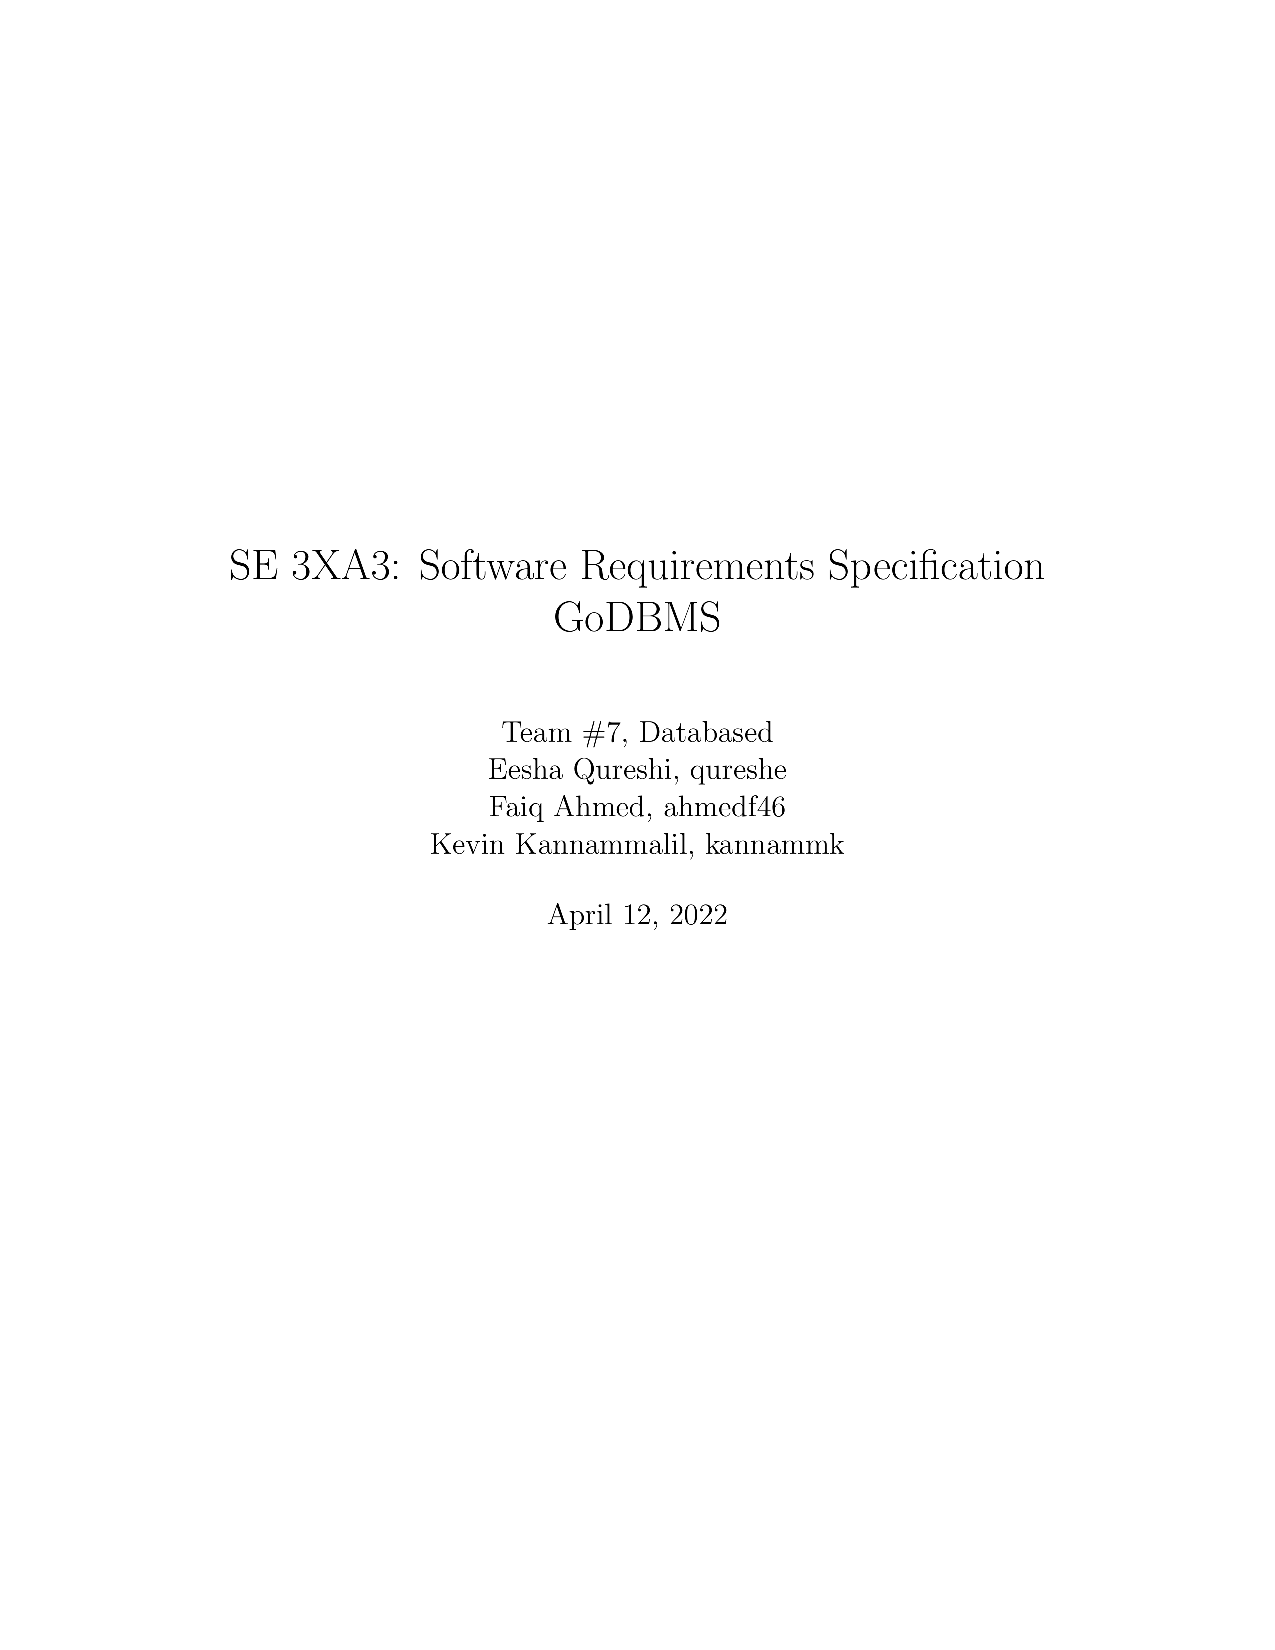
\includegraphics[width=\textwidth]{MG.png}
\caption{Use hierarchy among modules}
\label{FigUH}
\end{figure}

%\section*{References}

\bibliographystyle {plainnat}
\bibliography {MG}

\end{document}